\section{Reproducing the experiments} \label{sec:reproduce-expes}

All scripts can be found in the
batkube-test\footnote{\url{https://www.github.com/oar-team/batkube-test}} repository, under the
\texttt{scripts} repository. The exact commands used to run Batkube, the
scheduler and Batsim are described in the shell scripts. Running an experiment
on an emulated cluster can be done with
\texttt{real-clutser-experiment/main.go}, after starting a cluster with
\texttt{scripts/startup-cluster.sh}. Both of these scripts are shipped with a
help section. Finally, \texttt{swf-translate/swf-to-json.go} is the script used
to process swf workloads. It also has a help section.\\

Batsim is run with option \texttt{enable-compute-sharing}: for a reason
unknown, Kubernetes scheduler tends to over allocate resources in some cases
(especially with smaller jobs) which makes Batsim crash if this option is
disabled. Then, we must allow compute sharing even when it is not expected in
order to capture the scheduler behavior as precisely as possible.\\

\section{Batsim events handled by Batkube} \label{sec:batmsg-list}

Here are all the Batsim events that are handled by Batkube.

\subsubsection{From Batsim to the scheduler}

\paragraph{SIMULATION\_BEGINS}
contains information about the available resources in the cluster, with
Batsim's configuration.

\paragraph{SIMULATION\_ENDS}
is sent at the very end of the simulation: all jobs have finished, and no more
jobs are left in the queues. Batsim exits on this message.

\paragraph{JOB\_SUBMITTED}
notifies the scheduler that a new job has been submitted. It contains
information about the job type, id and specifications. We only consider jobs of
type \textit{delay} to simplify the models. Delay jobs specifications boil down
to the delay length, to which we add resource requests.

\paragraph{JOB\_COMPLETED}
notifies the scheduler that a job has ended, specifying the reason for it. We
only consider situations where all jobs complete correctly. Their state is then
always COMPLETED\_SUCCESSFULLY in our case.

\paragraph{REQUESTED\_CALL}
is an awnser to a CALL\_ME\_LATER event sent by the scheduler.

\subsubsection{From the scheduler to Batsim}

\paragraph{CALL\_ME\_LATER}
is an incentive from the scheduler for Batsim to wake up at a certain
timestamp. When the timestamp is reached in the simulation, Batsim will send a
REQUESTED\_CALL to the scheduler. In our case, this particular exchange will
serve as the base for time synchronisation between the scheduler and Batsim.

\paragraph{EXECUTE\_JOB}
is sent when the scheduler has made a decision. It contains the id of the job
at stake and the id of the resources it has been scheduled to.

\subsubsection{Bidirectional}

\paragraph{NOTIFY}
is used to send some information to the other peer. In our case, we use the
NOTIFY containing no\_more\_static\_job\_to\_submit to determine if the
simulation has ended: knowing that there are no more jobs susceptible to be
scheduled allow us to fast forward to the end of the simulation, thus saving
execution time.\\


\begin{figure}
	\begin{minted}{js}
{
  "now": 1024.24,
  "events": [
    {
      "timestamp": 1000,
      "type": "EXECUTE_JOB",
      "data": {
        "job_id": "workload!job_1234",
        "alloc": "1 2 4-8",
      }
    },
    {
      "timestamp": 1012,
      "type": "EXECUTE_JOB",
      "data": {
        "job_id": "workload!job_1235",
        "alloc": "12-100",
      }
    }
  ]
}
\end{minted}
\caption{Example of a Batsim message}
\label{fig:batmsg_ex}
\end{figure}

\begin{figure}
	\begin{minted}{js}
{
    "nb_res": 1,
    "jobs": [
	{"id":"1", "subtime":0, "res": 1, "profile": "delay10"},
	{"id":"2", "subtime":3.4, "res": 1, "profile": "delay10"}
    ],
    "profiles": {
	"delay10": {
	    "type": "delay",
	    "delay": 10,
	    "scheduler": "default",
	    "cpu": "1.5",
	    "memory": "500Mi"
	}
    }
}
	\end{minted}
	\caption{Example of a Batsim workload}
	\label{fig:bat_wl_ex}
\end{figure}

\section{Batsim integration with Kubernetes: other options} \label{sec:imp_levels}

Here are the options that were considered but not chosen for Batsim integration
with the Kubernetes ecosystem.

\subsubsection{In between the api and the kubelets}

This is the lowest level option. We position the simulator so as to simulate
just the infrastructure and avoid tampering with Kubernetes resource
management, which is done in their API. This approach would allow us to
effortlessly use any Kubernetes scheduler once their API is supported by
Batkube, and potentially produce the most accurate results. However,
interactions between the kubelets and the API are not documented because the
typical user is not supposed to have to deal with this part of Kubernetes. This
would hinder the development of Batkube because a reverse engineering process
would be required beforehand to understand the intricacies of internal
Kuberenetes exchanges.

\begin{figure}[h]
	\centering
	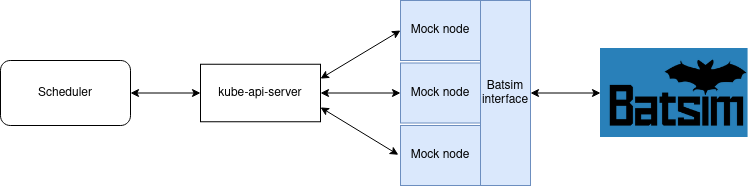
\includegraphics[width=\textwidth]{../imgs/architecture-as-kubelets.png}
	\caption{Mocking the cluster itself.}
	\label{fig:mock_nodes}
\end{figure}

\subsubsection{Custom client-go}

Most Kubernetes schedulers rely on
client-go\footnote{\url{https://github.com/kubernetes/client-go}}, which is a Go
client for the api-server. It is a library implementing various tools to help
schedulers converse with the API. By altering this client and patching
schedulers so they use our client instead, we can make it exchange with Batsim
instead of the API. 

\begin{figure}[h]
	\centering
	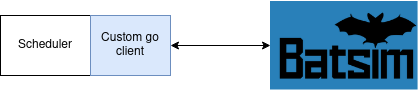
\includegraphics[scale=0.8]{../imgs/custom-go-client.png}
	\caption{Custom Go client to redirect scheduler communications to Batsim}
	\label{fig:custom-go-client}
\end{figure}

Contrary to the kubelets, client-go is a user interface and therefore it is
documented, facilitating reverse engineering of its source code. Still, it
represents thousands of lines of code and altering it to our needs would not be
an easy feat.  The other drawback to this approach is that Batkube would only
support schedulers written in Go and making use of client-go, although this
should not be an issue as the only kubernetes scheduler we could find that does
not rely on client-go is a toy scheduler written in
bash\footnote{\url{https://github.com/rothgar/bashScheduler}}.

\subsubsection{Partial reimplementation of the API}

Re-implementing the API offers a middle ground between the low level and
undocumented solution of the mock nodes, and the higher level and technically
challenging solution of a client-go fork. Again, there are several options here.

A partial reimplementation of the API would save us the task of building a new
API from the ground up. However this would imply digging deep into the
api-server code in order to understand how the api is organized and what code
we would have to alter. In the end, it is easier to simply build a new API,
since there are tools to help us generate it from its specification.

\begin{figure}[h]
	\centering
	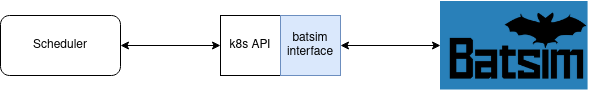
\includegraphics[scale=0.8]{../imgs/partial-reimplem.png}
	\caption{Partial reimplementation of the api-server.}
	\label{fig:partial_reimp}
\end{figure}

\section{Time interception: the C library approach}

An attempt was first made to patch a custom C library, which is the lowest level
solution. Going for the low level solution would truly redirect all calls to
machine time which is something we can not guarantee with the second option, as
we explain in section \ref{sec:patch-scheds}. This approach proved challenging
due to circular dependency issues and was ultimately abandoned. We opted for
the second option which consist of modifying Go source code, which requires
some additional work to patch the schedulers but was actually easier to
implement.

\begin{figure}
	\centering
	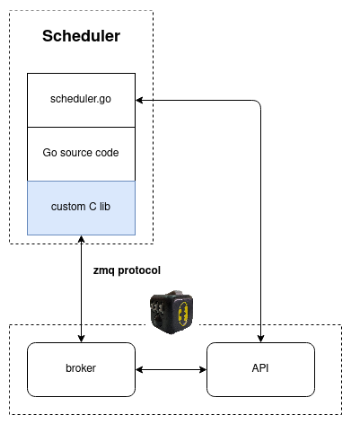
\includegraphics[scale=0.5]{../imgs/time-hijack-C.png}
	\caption{Option A: patching the C library}
	\label{fig:patch-C}
\end{figure}
